\begin{appendices}

    \chapter{Forms and Questionnaires}

    \section{Public Opinion Survey}
    \label{app:public-opinion-survey}

    \begin{center}
        \begin{tcolorbox}[breakable, colback=white, colframe=black, width=\textwidth, boxrule=0.5pt]
            \scriptsize

            \textbf{Demographic Information}
            \begin{enumerate}
                \item What is your age range?
                \item What is your gender?
                \item What is your race/ethnicity? (Select all that apply)
                \item Which of the following best describes your current workplace environment? (Select all that apply)
                \item Do you have any mobility impairments that affect how you interact with access control systems?
            \end{enumerate}

            \textbf{Current Experience with Access Control}
            \begin{enumerate}
                \item Which of the following physical access control methods do you have experience using? (Select all that apply)
                \item On a scale of 1-5, how satisfied are you with your current access control method(s)? (1 = Very dissatisfied, 5 = Very satisfied)
                \item Have you ever experienced any of the following issues with access control methods?
                \item If you've used biometric authentication (fingerprint, face, iris), have you noticed any inconsistencies in performance based on:
                \item Are you aware of, or have you experienced any cases where an access control system has shown bias/discrimination or has failed to work for you while working for others?
                \item If you selected Yes to the previous question, please describe the case(s) you have witnessed and/or experienced.
            \end{enumerate}

            \textbf{Preferences and Priorities}
            \begin{enumerate}
                \item Rate the importance of the following factors in access control systems (1-5 scale):
                      \begin{itemize}
                          \item Speed and Convenience
                          \item Security Level
                          \item Privacy Protection
                          \item Not having to carry additional items
                          \item Reliability in different conditions
                      \end{itemize}
                \item Which of the following best describes your interaction preferences with access control systems?
            \end{enumerate}

            \textbf{Security Perceptions}
            \begin{enumerate}
                \item Rate the perceived security level of the following access methods (1-5 scale):
                      \begin{itemize}
                          \item RFID/key cards
                          \item PIN codes
                          \item Fingerprint recognition
                          \item Facial recognition
                          \item Gait recognition
                      \end{itemize}
            \end{enumerate}

            \textbf{Gait Recognition Specific Questions}
            \begin{enumerate}
                \item How comfortable would you be with a system that authenticates you based on your walking style (gait) as you approach a door?
                \item Which of the following would increase your comfort with biometric authentication systems?
                \item How would you prefer to be authenticated in the future?
                \item Would you be willing to participate in the enrollment process (providing initial data) for a gait recognition system if it meant more convenient access afterward?
            \end{enumerate}

            \textbf{Additional Comments}
            \begin{enumerate}
                \item Have you experienced any access control issues that weren't covered in this survey?
                \item Do you have any additional comments, concerns, or suggestions regarding physical access control systems?
            \end{enumerate}
        \end{tcolorbox}
    \end{center}


    \section{Participant Information Sheet}
    \label{app:participant-information-sheet}

    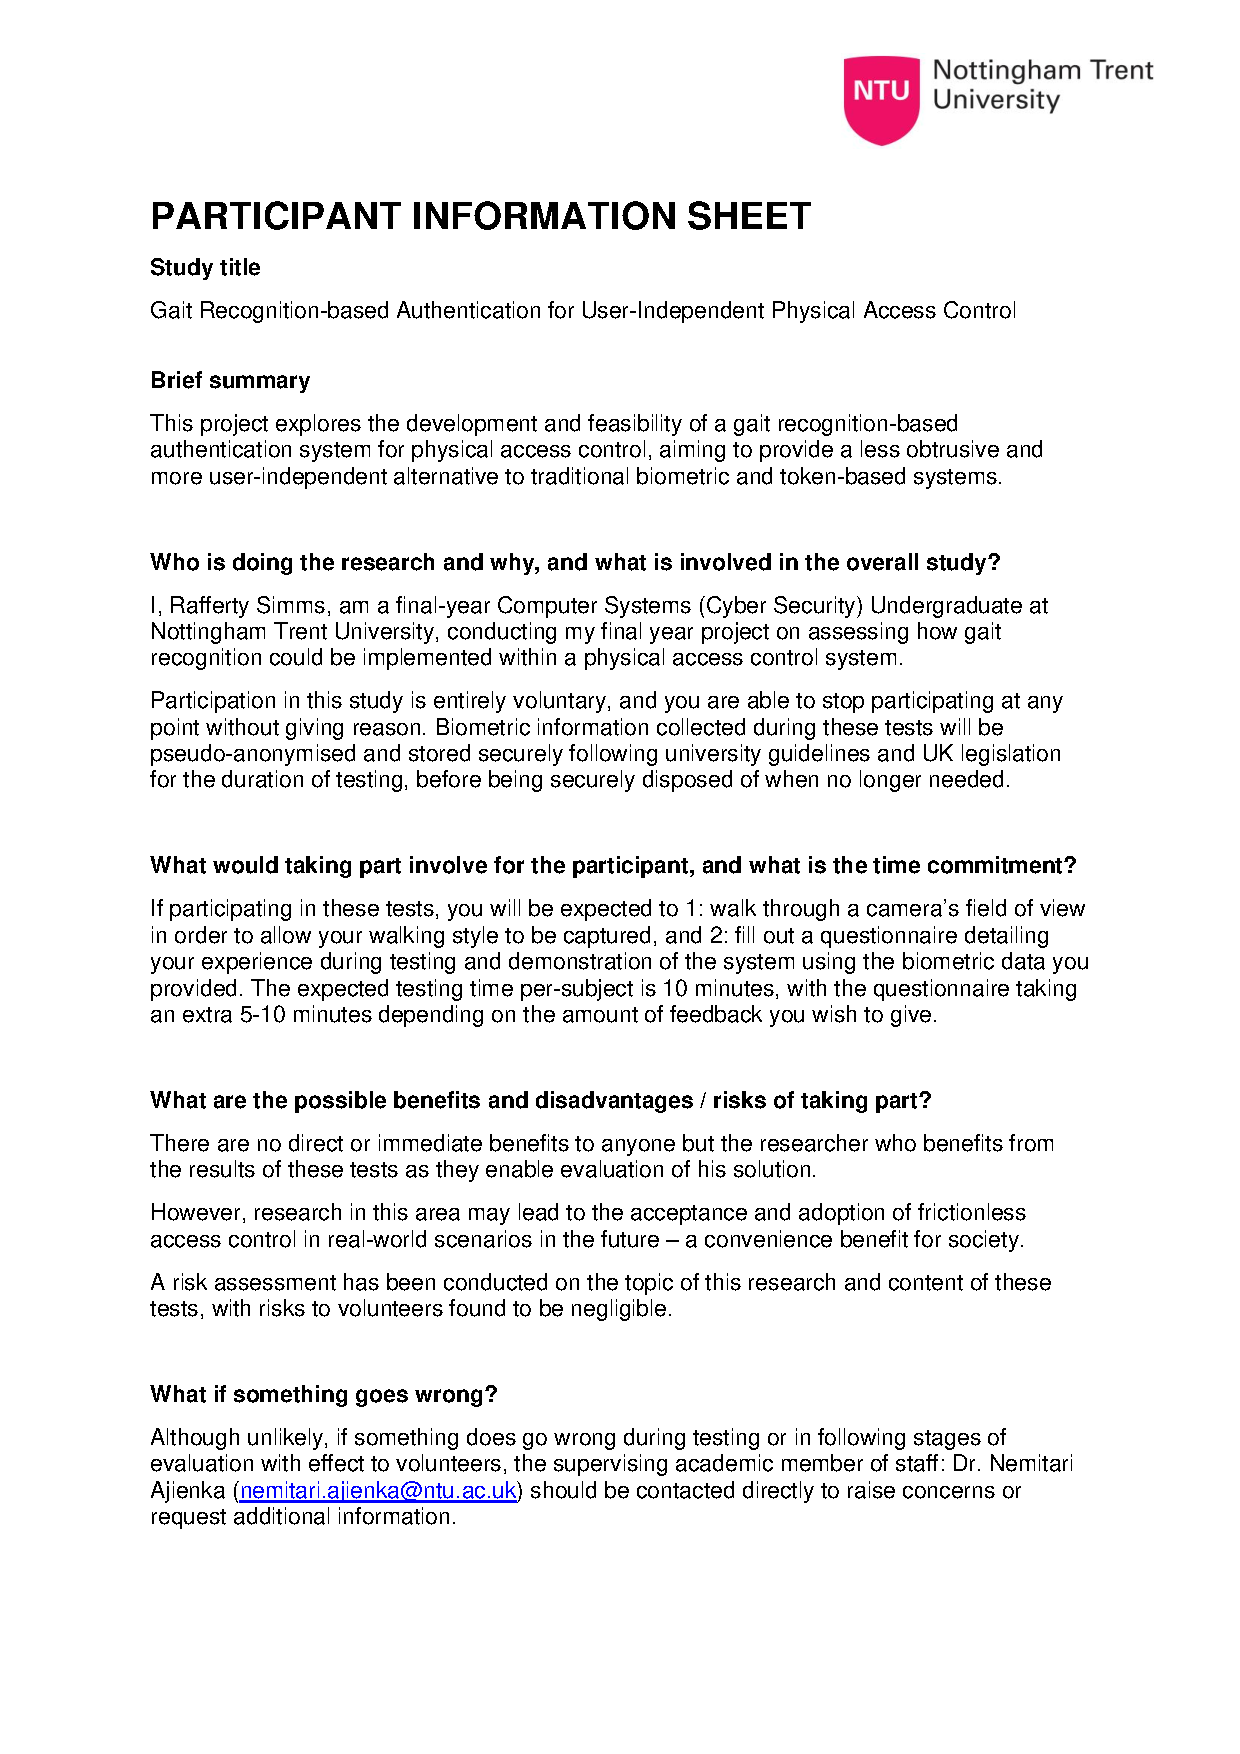
\includepdf[pages=-,width=\textwidth, height=\textheight, keepaspectratio]{assets/pis.pdf}

    \section{Informed Consent Form}
    \label{app:informed-consent-form}

    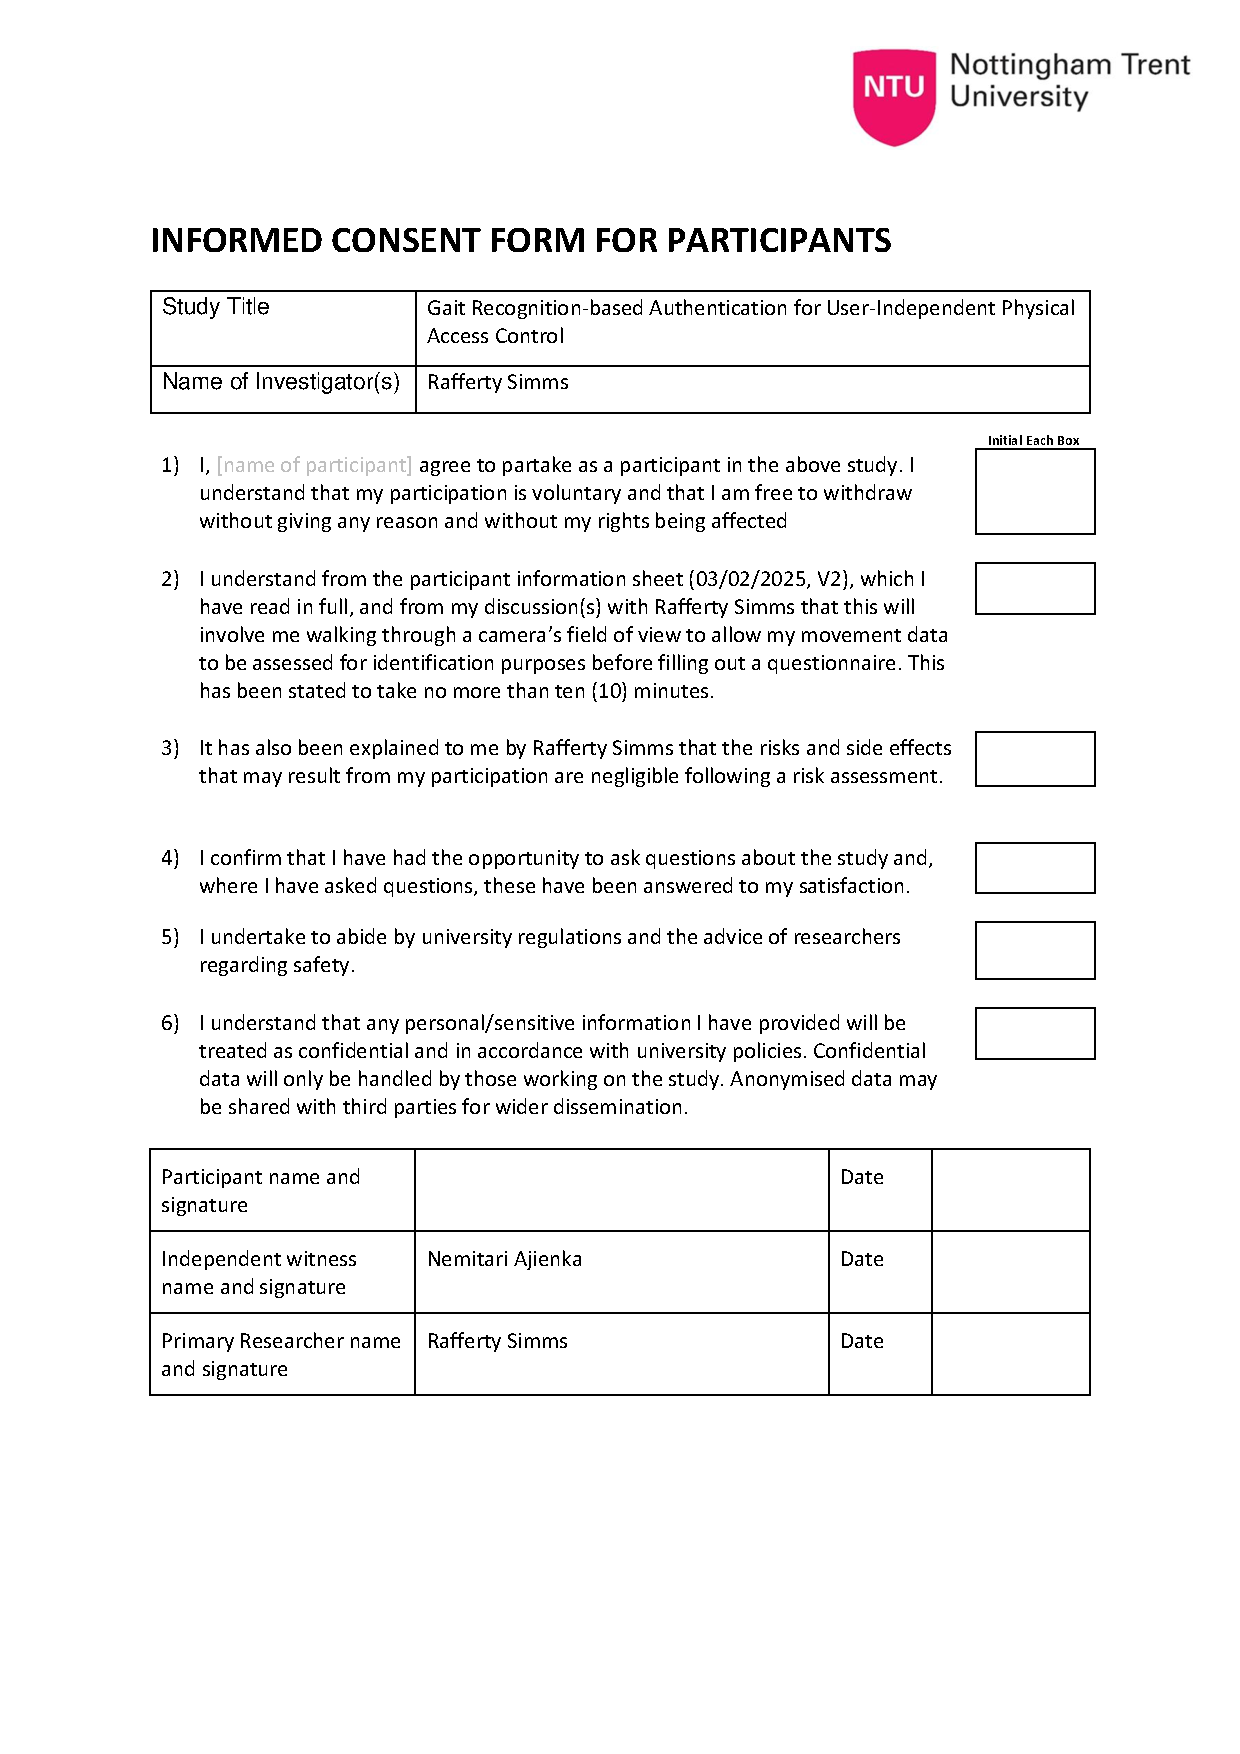
\includegraphics[width=\textwidth, height=\textheight, keepaspectratio]{assets/ic.pdf}

    \chapter{Risk Assessment Matrix}
    \label{app:risk-assessment-matrix}

    \begin{figure}[H]
        \centering
        \rotatebox{90}{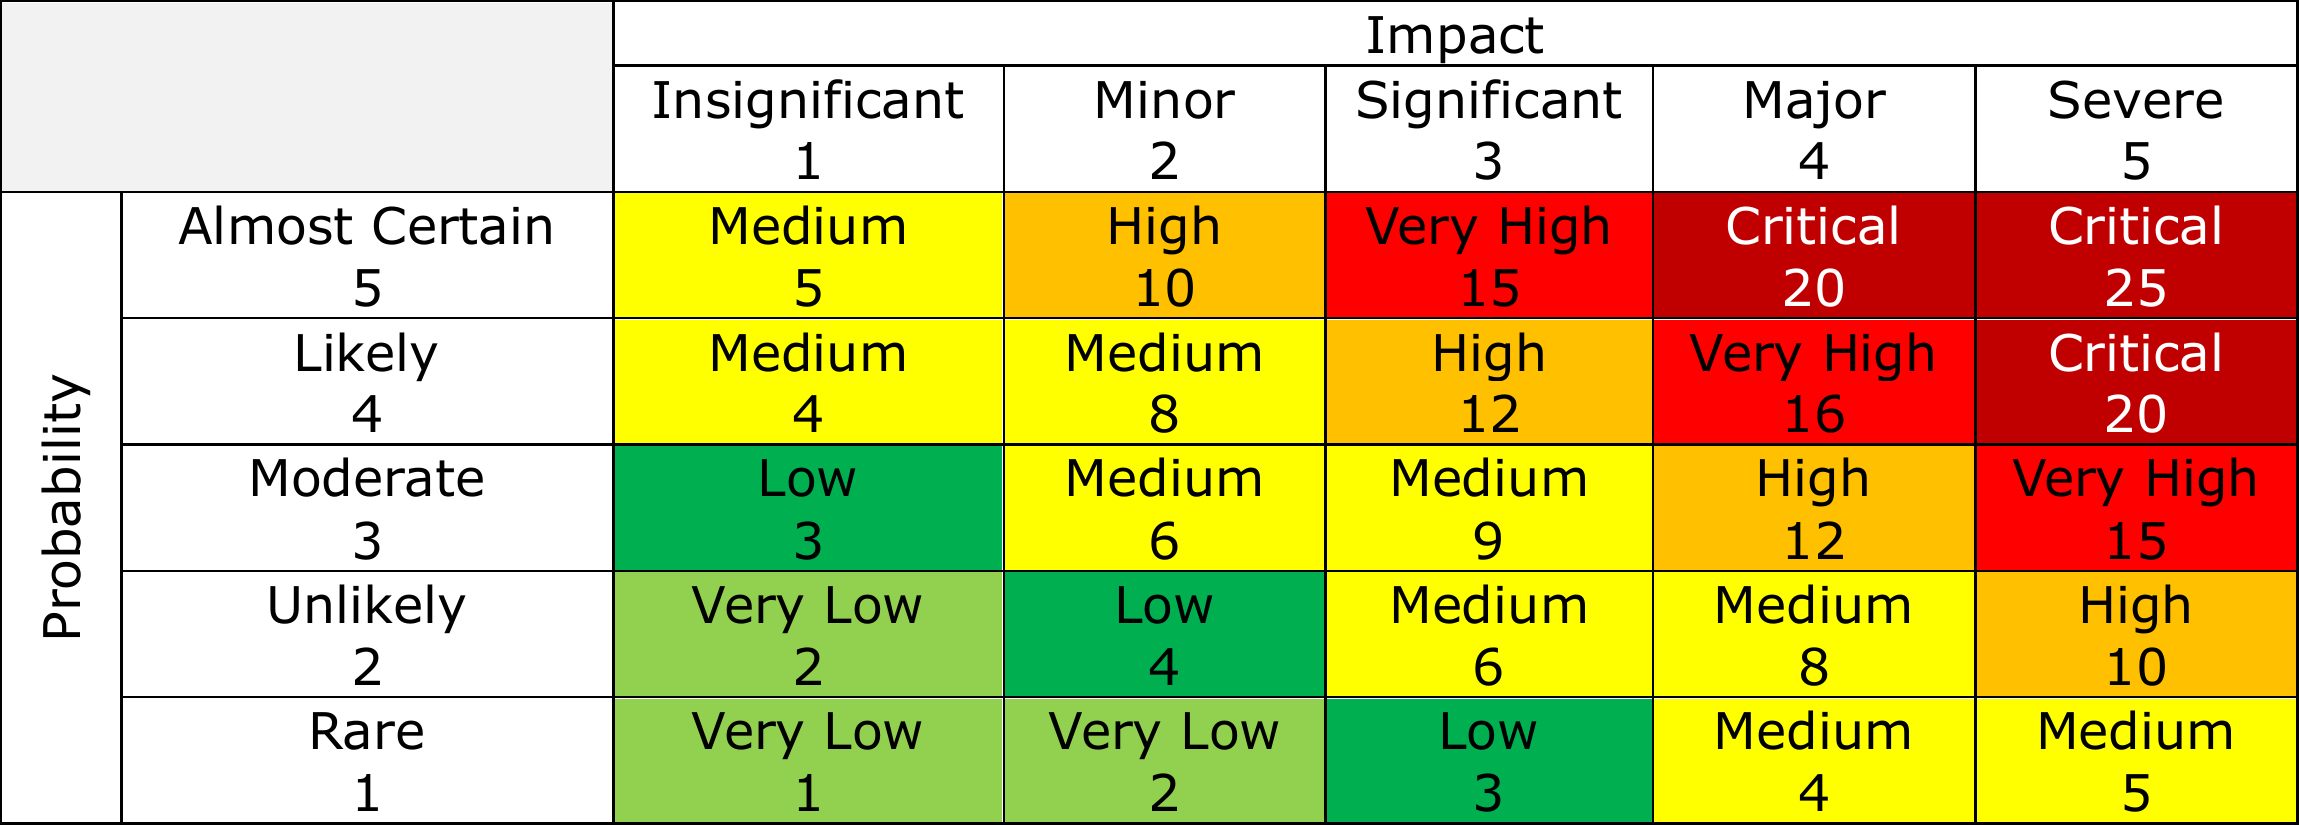
\includegraphics[width=0.8\textheight, keepaspectratio]{assets/risk_assessment_matrix.png}}
    \end{figure}

    \chapter{Implementation}

    \section{Code Extracts}

    \subsection{The 'Camera' Class}
    \label{app:camera-implementation}

    \begin{code}
class Camera:
    def __init__(self, camera_id=0):
        self.camera_id = camera_id
        self.cap = None
        self.is_running = False
        self.current_frame = None
        self.lock = threading.Lock()

    def start(self):
        if self.is_running:
            return

        self.cap = cv2.VideoCapture(self.camera_id)
        if not self.cap.isOpened():
            raise ValueError(f"Failed to open camera {self.camera_id}")

        self.is_running = True
        self.thread = threading.Thread(target=self._capture)
        self.thread.daemon = True
        self.thread.start()

    def stop(self):
        self.is_running = False
        if self.thread:
            self.thread.join()
        if self.cap:
            self.cap.release()

    def _capture(self):
        while self.is_running:
            ret, frame = self.cap.read()
            if ret:
                with self.lock:
                    self.current_frame = frame
            time.sleep(0.01)

    def get_frame(self):
        with self.lock:
            if self.current_frame is None:
                return None
            return self.current_frame.copy()
    \end{code}

    \subsection{The 'GaitProcessor' Class}
    \label{app:gait-processor-implementation}
    \noindent
    \begin{code}
class GaitProcessor:
    NORMALISED_WIDTH = 88
    NORMALISED_HEIGHT = 128
    MIN_CONTOUR_AREA = 500
    MIN_ASPECT_RATIO = 1.5
    MAX_ASPECT_RATIO = 3.5

    def __init__(self, initial_frames=30, buffer_size=30, alpha=0.2):
        self.background_model = None
        self.initial_frames_count = initial_frames
        self.background_frames = []
        self.buffer_size = buffer_size
        self.alpha = alpha
        self.aligned_buffer = deque(maxlen=buffer_size) if buffer_size > 0 else []
        self.aligned_gei = None

    def initialise_backround(self, frame):
        gray = cv2.cvtColor(frame, cv2.COLOR_BGR2GRAY)
        self.background_frames.append(gray)

        if len(self.background_frames) >= self.initial_frames_count:
            self.background_model = np.median(self.background_frames, axis=0).astype(
                np.uint8
            )
            self.background_frames = []
            return True

        return False

    def reset_background(self):
        self.background_model = None
        self.background_frames.clear()
        self.aligned_gei = None
        self.aligned_buffer.clear()

    def process_frame(self, frame):
        if self.background_model is None:
            return None, None

        silhouette, bounding_box = self._extract_silhouette(frame)

        if bounding_box is not None:
            self._draw_bounding_box(frame, bounding_box)

            aligned_silhouette = self._align_silhouette(silhouette, bounding_box)
            if aligned_silhouette is not None:
                self._update_gei(aligned_silhouette)

        if self.aligned_gei is not None:
            gei = (self.aligned_gei * 255).astype(np.uint8)
        else:
            gei = np.zeros(
                (self.NORMALISED_HEIGHT, self.NORMALISED_WIDTH), dtype=np.uint8
            )

        return silhouette, gei

    def _extract_silhouette(self, frame):
        gray = cv2.cvtColor(frame, cv2.COLOR_BGR2GRAY)
        gray = cv2.GaussianBlur(gray, (3, 3), 0)

        diff = cv2.absdiff(self.background_model, gray)
        _, binary = cv2.threshold(diff, 25, 255, cv2.THRESH_BINARY)

        silhouette = cv2.morphologyEx(
            binary, cv2.MORPH_CLOSE, np.ones((5, 5), np.uint8)
        )

        contours, _ = cv2.findContours(
            silhouette, cv2.RETR_EXTERNAL, cv2.CHAIN_APPROX_SIMPLE
        )
        large_contours = [
            cnt for cnt in contours if cv2.contourArea(cnt) > self.MIN_CONTOUR_AREA
        ]

        filtered_silhouette = np.zeros_like(silhouette)
        cv2.drawContours(filtered_silhouette, large_contours, -1, 255, -1)

        bounding_box = None
        if large_contours:
            largest_contour = max(large_contours, key=cv2.contourArea)
            x, y, w, h = cv2.boundingRect(largest_contour)

            aspect_ratio = h / w
            if self.MIN_ASPECT_RATIO <= aspect_ratio <= self.MAX_ASPECT_RATIO:
                bounding_box = (x, y, w, h)

        return filtered_silhouette, bounding_box

    def _align_silhouette(self, silhouette, bounding_box):
        x, y, w, h = bounding_box

        person_region = silhouette[y : y + h, x : x + w]

        ty, tx = np.where(person_region > 0)

        if len(ty) == 0 or len(tx) == 0:
            return None

        sy, ey = ty.min(), ty.max() + 1
        sx, ex = tx.min(), tx.max() + 1

        silhouette_h = ey - sy
        silhouette_w = ex - sx

        if silhouette_h <= silhouette_w:
            return None

        cx = int(tx.mean())
        cenX = silhouette_h // 2
        start_w = (silhouette_h - silhouette_w) // 2

        if max(cx - sx, ex - cx) < cenX:
            start_w = cenX - (cx - sx)

        square_silhouette = np.zeros((silhouette_h, silhouette_h), np.uint8)
        square_silhouette[:, start_w : start_w + silhouette_w] = person_region[
            sy:ey, sx:ex
        ]

        resized_silhouette = cv2.resize(
            square_silhouette,
            (self.NORMALISED_HEIGHT, self.NORMALISED_HEIGHT),
            interpolation=cv2.INTER_AREA,
        )

        offsetX = 20
        normalised_silhouette = resized_silhouette[
            :, offsetX : offsetX + self.NORMALISED_WIDTH
        ]

        return normalised_silhouette.astype(float) / 255.0

    def _update_gei(self, aligned_silhouette):
        self.aligned_buffer.append(aligned_silhouette)

        if self.buffer_size == 0 or len(self.aligned_buffer) == self.buffer_size:
            if self.aligned_gei is None:
                self.aligned_gei = np.mean(self.aligned_buffer, axis=0)
            else:
                new_gei = np.mean(self.aligned_buffer, axis=0)
                self.aligned_gei = (
                    1 - self.alpha
                ) * self.aligned_gei + self.alpha * new_gei
    \end{code}

    \subsection{Client-Side Identity Classification Thread}
    \label{app:identity-classification-thread-implementation}

    \begin{code}
def classification_thread():
    while True:
        if state["frame_counter"] >= FRAME_INTERVAL:
            current_gei = state["gei_buffer"]
            last_saved_gei = state["last_saved_gei"]

            if current_gei is not None:
                if is_different(current_gei, last_saved_gei):

                    _, buffer = cv2.imencode(".jpg", current_gei)
                    gei_base64 = base64.b64encode(buffer).decode("utf-8")

                    state["last_saved_gei"] = current_gei

                    response, message = api_client.classify_gei(gei_base64)
                    print(response)
                    if not response:
                        print(f"Failed to classify GEI: {message}")
                    else:
                        socketio.emit("status", response)

            state["frame_counter"] = 0

        time.sleep(1)
    \end{code}

    \subsection{SQLAlchemy Database Models}
    \label{app:database-models-implementation}

    \begin{code}
class Identity(db.Model):
    __tablename__ = "Identities"
    id = db.Column(db.Integer, primary_key=True)
    label = db.Column(db.String(50), nullable=False)
    gait_samples = db.relationship(
        "GaitSample", backref="identity", lazy=True, cascade="all, delete-orphan"
    )
    access_rule = db.relationship(
        "AccessRule",
        backref="identity",
        lazy=True,
        uselist=False,
        cascade="all, delete-orphan",
    )


class GaitSample(db.Model):
    __tablename__ = "GaitSamples"
    id = db.Column(db.Integer, primary_key=True)
    identity_id = db.Column(db.Integer, db.ForeignKey("Identities.id"), nullable=False)
    gei_image = db.Column(db.Text, nullable=False)
    features = db.Column(db.LargeBinary, nullable=False)
    created_at = db.Column(db.DateTime, default=datetime.now)


class AccessRule(db.Model):
    __tablename__ = "AccessRules"
    identity_id = db.Column(
        db.Integer, db.ForeignKey("Identities.id"), primary_key=True
    )
    rule = db.Column(db.Boolean, nullable=False, default=False)


class GaitModel(db.Model):
    __tablename__ = "GaitModels"
    id = db.Column(db.Integer, primary_key=True)
    pca_components = db.Column(db.LargeBinary, nullable=False)
    mean_vector = db.Column(db.LargeBinary, nullable=False)
    n_components = db.Column(db.Integer, nullable=False)
    created_at = db.Column(db.DateTime, default=datetime.now)
    updated_at = db.Column(db.DateTime, default=datetime.now, onupdate=datetime.now)


class ActivityLog(db.Model):
    __tablename__ = "ActivityLogs"
    id = db.Column(db.Integer, primary_key=True)
    activity_type = db.Column(db.String(20), nullable=False)
    details = db.Column(db.Text, nullable=True)
    created_at = db.Column(db.DateTime, default=datetime.now)
    \end{code}

    \subsection{Activity Log Retrieval and Formatting}
    \label{app:activity-log-retrieval-and-formatting}

    \begin{code}
recent_activity = ActivityLog.query.order_by(ActivityLog.created_at.desc()).all()

formatted_logs = []
for log in recent_activity:
    timestamp = log.created_at.strftime("%Y-%m-%d %H:%M:%S")
    details = eval(log.details) if log.details else {}

    if log.activity_type == "register":
        label = details.get("label", "Unknown")
        message = f"Registered new gait sample for {label}"
    elif log.activity_type == "delete":
        label = details.get("label", "Unknown")
        if details.get("type") == "identity":
            message = f"Deleted identity: {label}"
        else:
            message = f"Deleted gait sample for {label}"
    elif log.activity_type == "access_change":
        label = details.get("label", "Unknown")
        new_state = "granted" if details.get("new_state") else "denied"
        message = f"Access {new_state} for {label}"
    elif log.activity_type == "identify":
        label = details.get("label", "Unknown")
        confidence = details.get("confidence", 0)
        message = f"Identified as {label} (confidence: {confidence}%)"
    else:
        message = f"Unknown activity"

    formatted_logs.append(
        {"timestamp": timestamp, "message": message, "type": log.activity_type}
    )
    \end{code}

    \section{Client Code Architecture Diagram}
    \label{app:client-code-architecture}

    \begin{figure}[H]
        \centering
        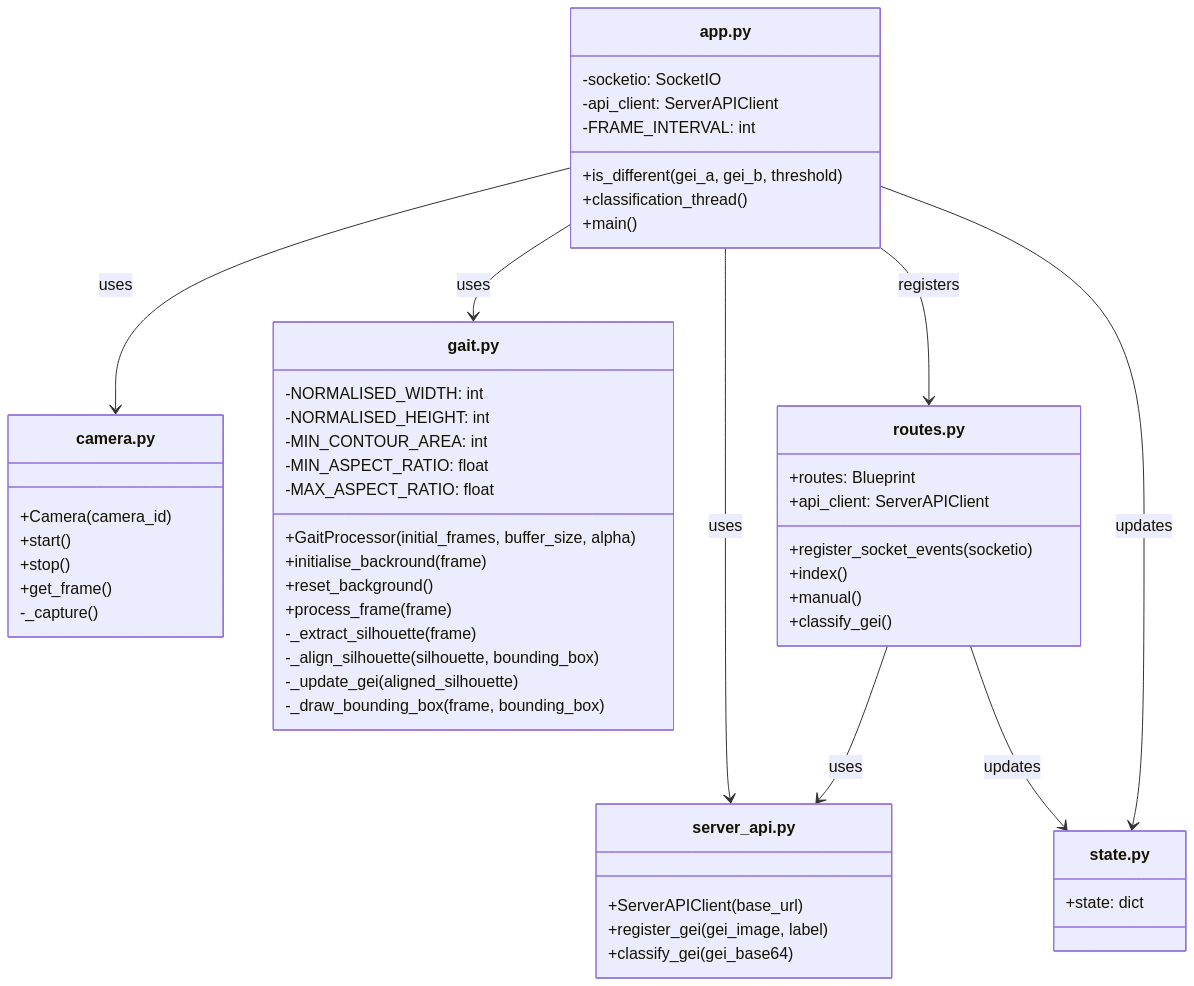
\includegraphics[width=\textwidth]{assets/client_architecture.png}
    \end{figure}

    \section{Server Code Architecture Diagram}
    \label{app:server-code-architecture}

    \begin{figure}[H]
        \centering
        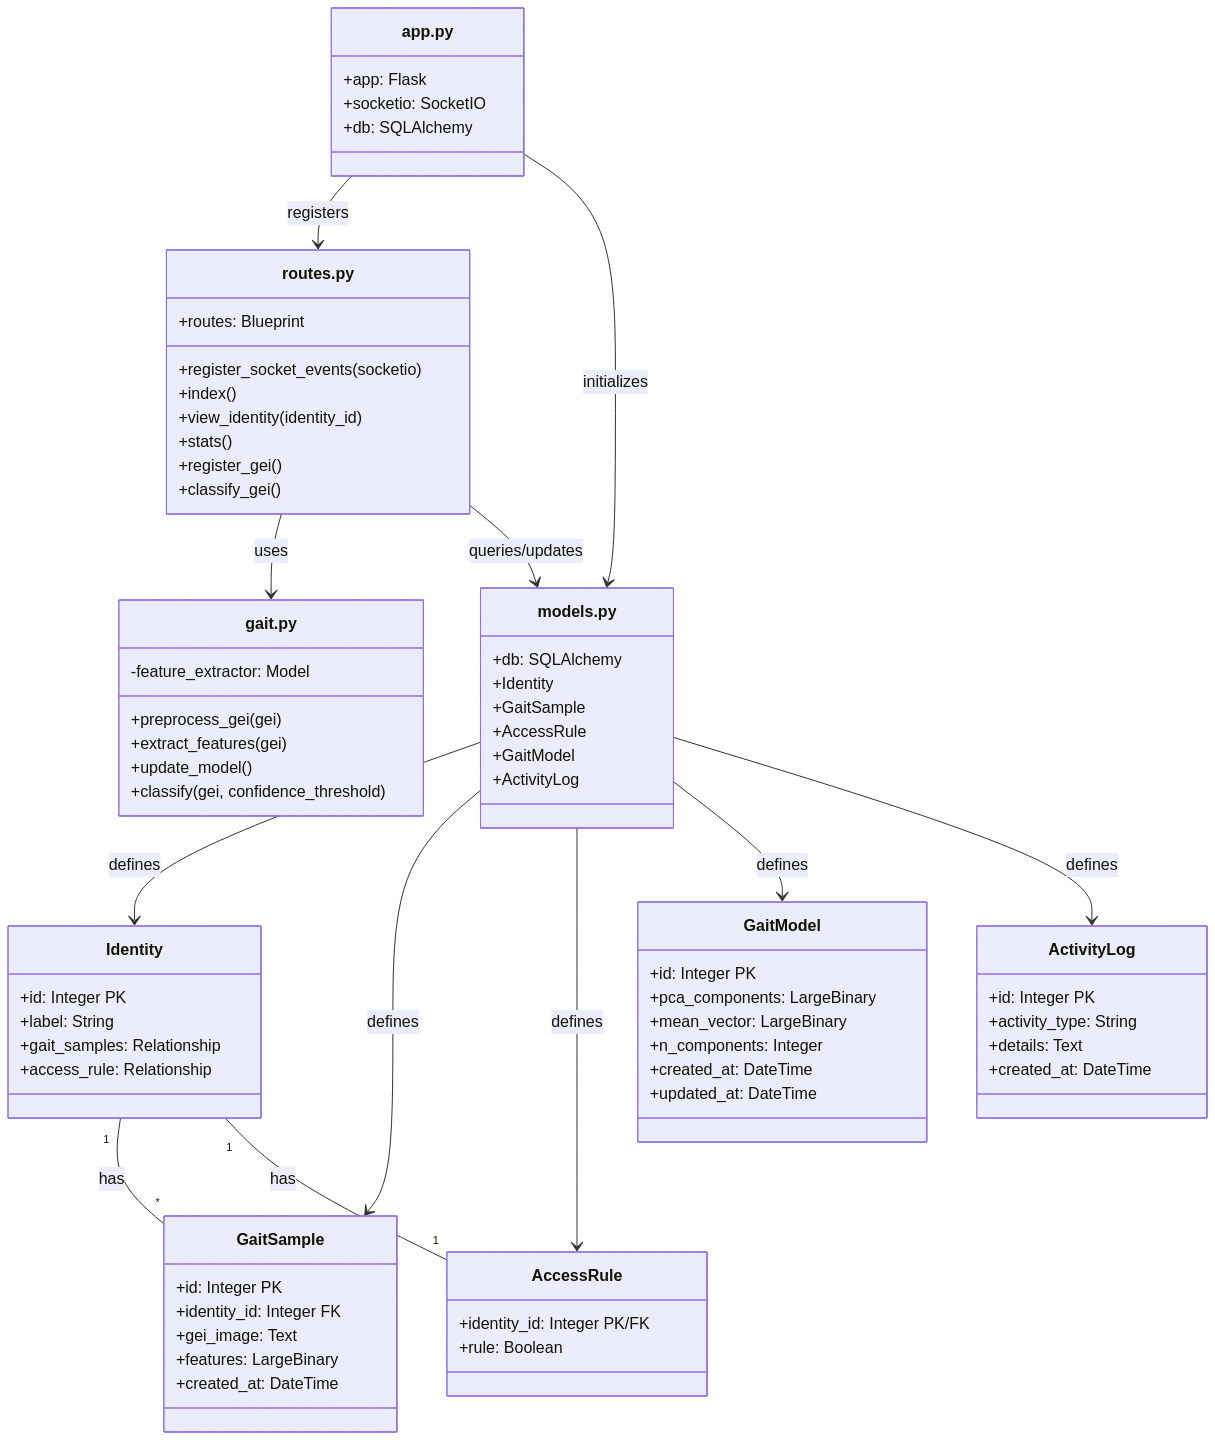
\includegraphics[width=\textwidth]{assets/server_architecture.png}
    \end{figure}
    
    \chapter{Training and Testing Automation}

    \section{Automated Registration Submission Function}
    \label{app:gait-recognition-server-training-function}

    \begin{code}
LOG_FILE = "registration_times.csv"

def submit_gei_to_api(gei_dir, api_url):
    gei_files = [f for f in os.listdir(gei_dir)]

    if not os.path.exists(LOG_FILE):
        with open(LOG_FILE, "w") as f:
            f.write("timestamp,file,subject_id,response_time,status\n")

    for gei_file in tqdm(gei_files):
        gei_path = os.path.join(gei_dir, gei_file)
        subject_id = gei_file[:3]

        with open(gei_path, "rb") as img_file:
            encoded_image = base64.b64encode(img_file.read()).decode("utf-8")

        data = {"gei": encoded_image, "label": subject_id}

        start_time = time.time()
        response = requests.post(api_url, json=data)
        end_time = time.time()
        response_time = end_time - start_time

        timestamp = datetime.datetime.now().isoformat()

        if response.status_code == 200:
            status = "success"
        else:
            status = f"error_{response.status_code}"

        with open(LOG_FILE, "a") as log_file:
            ... Write Log Entry
    \end{code}

    \section{Automated Classification Query Function}
    \label{app:gait-recognition-server-testing-function}

    \begin{code}
def test_gei_classification(test_dir, api_url):
    gei_files = [f for f in os.listdir(test_dir)]
    results = []

    for gei_file in tqdm(gei_files):
        gei_path = os.path.join(test_dir, gei_file)

        true_label = gei_file[:3]

        with open(gei_path, "rb") as img_file:
            encoded_image = base64.b64encode(img_file.read()).decode("utf-8")

        data = {"gei": encoded_image}

        start_time = time.time()
        response = requests.post(api_url, json=data)
        end_time = time.time()
        response_time = end_time - start_time

        if response.status_code == 200:
            result = response.json()
            predicted_label = result.get("person")
            confidence = result.get("confidence", 0)

            results.append(
                {
                    "file": gei_file,
                    "true_label": true_label,
                    "predicted_label": predicted_label,
                    "confidence": confidence,
                    "correct": predicted_label == true_label,
                    "above_threshold": confidence >= 75.0,
                    "response_time": response_time,
                }
            )
        else:
            ... Error Entry

    with open("classification_results.json", "w") as out:
        json.dump(results, out)
    \end{code}

    \chapter{Project Proposal Document LESPIs}
    \label{app:original-legal-ethical-social-and-professional-issues}

    
\includegraphics[page=9, trim=0 0 0 0.75\paperheight, clip, width=\textwidth, height=\textheight, keepaspectratio]{assets/N0990815_PPD.pdf}

    % Allow automatic breaking and include pages 5-8 as scaled images
    
\includegraphics[page=10, width=\textwidth, height=\textheight, keepaspectratio]{assets/N0990815_PPD.pdf}
    
    
\includegraphics[page=11, width=\textwidth, height=\textheight, keepaspectratio]{assets/N0990815_PPD.pdf}
    
    
\includegraphics[page=12, width=\textwidth, height=\textheight, keepaspectratio]{assets/N0990815_PPD.pdf}
    
    
\includegraphics[page=13, width=\textwidth, height=\textheight, keepaspectratio]{assets/N0990815_PPD.pdf}
\end{appendices}

